% !TeX program = pdflatex
% !TeX root = TID.tex

\documentclass[../FeynCalcManual.tex]{subfiles}
\begin{document}
\hypertarget{tid}{
\section{TID}\label{tid}\index{TID}}

\texttt{TID[\allowbreak{}amp,\ \allowbreak{}q]} performs tensor
decomposition of 1-loop integrals with loop momentum \texttt{q}.

\subsection{See also}

\hyperlink{toc}{Overview}, \hyperlink{oneloopsimplify}{OneLoopSimplify},
\hyperlink{tidl}{TIDL}, \hyperlink{pavelimitto4}{PaVeLimitTo4}.

\subsection{Examples}

\begin{Shaded}
\begin{Highlighting}[]
\NormalTok{FCClearScalarProducts}\OperatorTok{[]}\NormalTok{;}
\end{Highlighting}
\end{Shaded}

\begin{Shaded}
\begin{Highlighting}[]
\NormalTok{int }\ExtensionTok{=}\NormalTok{ FAD}\OperatorTok{[\{}\FunctionTok{k}\OperatorTok{,} \FunctionTok{m}\OperatorTok{\},} \FunctionTok{k} \SpecialCharTok{{-}} \FunctionTok{Subscript}\OperatorTok{[}\FunctionTok{p}\OperatorTok{,} \DecValTok{1}\OperatorTok{],} \FunctionTok{k} \SpecialCharTok{{-}} \FunctionTok{Subscript}\OperatorTok{[}\FunctionTok{p}\OperatorTok{,} \DecValTok{2}\OperatorTok{]]}\NormalTok{ FVD}\OperatorTok{[}\FunctionTok{k}\OperatorTok{,} \SpecialCharTok{\textbackslash{}}\OperatorTok{[}\NormalTok{Mu}\OperatorTok{]]} \SpecialCharTok{//}\NormalTok{ FCI}
\end{Highlighting}
\end{Shaded}

\begin{dmath*}\breakingcomma
\frac{k^{\mu }}{\left(k^2-m^2\right).(k-p_1){}^2.(k-p_2){}^2}
\end{dmath*}

By default, all tensor integrals are reduced to the Passarino-Veltman
scalar integrals \(A_0\), \(B_0\), \(C_0\), \(D_0\) etc.

\begin{Shaded}
\begin{Highlighting}[]
\NormalTok{TID}\OperatorTok{[}\NormalTok{int}\OperatorTok{,} \FunctionTok{k}\OperatorTok{]}
\end{Highlighting}
\end{Shaded}

\begin{dmath*}\breakingcomma
\frac{p_1{}^2 p_2{}^{\mu }-p_1{}^{\mu } \left(p_1\cdot p_2\right)}{2 \left((p_1\cdot p_2){}^2-p_1{}^2 p_2{}^2\right) k^2.\left((k+p_1){}^2-m^2\right)}-\frac{p_2{}^2 \left(m^2+p_1{}^2\right) p_1{}^{\mu }+p_1{}^2 \left(m^2+p_2{}^2\right) p_2{}^{\mu }+\left(m^2+p_1{}^2\right) \left(-p_2{}^{\mu }\right) \left(p_1\cdot p_2\right)-\left(m^2+p_2{}^2\right) p_1{}^{\mu } \left(p_1\cdot p_2\right)}{2 \left((p_1\cdot p_2){}^2-p_1{}^2 p_2{}^2\right) \left(k^2-m^2\right).(k-p_1){}^2.(k-p_2){}^2}-\frac{p_2{}^{\mu } \left(p_1\cdot p_2\right)-p_2{}^2 p_1{}^{\mu }}{2 \left((p_1\cdot p_2){}^2-p_1{}^2 p_2{}^2\right) k^2.\left((k+p_2){}^2-m^2\right)}-\frac{p_1{}^2 p_2{}^{\mu }+p_2{}^2 p_1{}^{\mu }-p_1{}^{\mu } \left(p_1\cdot p_2\right)-p_2{}^{\mu } \left(p_1\cdot p_2\right)}{2 k^2.(k-p_1+p_2){}^2 \left((p_1\cdot p_2){}^2-p_1{}^2 p_2{}^2\right)}
\end{dmath*}

Scalar integrals can be converted to the Passarino-Veltman notation via
the option \texttt{ToPaVe}

\begin{Shaded}
\begin{Highlighting}[]
\NormalTok{TID}\OperatorTok{[}\NormalTok{int}\OperatorTok{,} \FunctionTok{k}\OperatorTok{,}\NormalTok{ ToPaVe }\OtherTok{{-}\textgreater{}} \ConstantTok{True}\OperatorTok{]}
\end{Highlighting}
\end{Shaded}

\begin{dmath*}\breakingcomma
\frac{i \pi ^2 \left(p_1{}^2 p_2{}^{\mu }-p_1{}^{\mu } \left(p_1\cdot p_2\right)\right) \;\text{B}_0\left(p_1{}^2,0,m^2\right)}{2 \left((p_1\cdot p_2){}^2-p_1{}^2 p_2{}^2\right)}-\frac{i \pi ^2 \left(p_2{}^{\mu } \left(p_1\cdot p_2\right)-p_2{}^2 p_1{}^{\mu }\right) \;\text{B}_0\left(p_2{}^2,0,m^2\right)}{2 \left((p_1\cdot p_2){}^2-p_1{}^2 p_2{}^2\right)}-\frac{i \pi ^2 \left(p_1{}^2 p_2{}^{\mu }+p_2{}^2 p_1{}^{\mu }-p_1{}^{\mu } \left(p_1\cdot p_2\right)-p_2{}^{\mu } \left(p_1\cdot p_2\right)\right) \;\text{B}_0\left(p_1{}^2-2 \left(p_1\cdot p_2\right)+p_2{}^2,0,0\right)}{2 \left((p_1\cdot p_2){}^2-p_1{}^2 p_2{}^2\right)}-\frac{i \pi ^2 \left(p_2{}^2 \left(m^2+p_1{}^2\right) p_1{}^{\mu }+p_1{}^2 \left(m^2+p_2{}^2\right) p_2{}^{\mu }+\left(m^2+p_1{}^2\right) \left(-p_2{}^{\mu }\right) \left(p_1\cdot p_2\right)-\left(m^2+p_2{}^2\right) p_1{}^{\mu } \left(p_1\cdot p_2\right)\right) \;\text{C}_0\left(p_1{}^2,p_2{}^2,p_1{}^2-2 \left(p_1\cdot p_2\right)+p_2{}^2,0,m^2,0\right)}{2 \left((p_1\cdot p_2){}^2-p_1{}^2 p_2{}^2\right)}
\end{dmath*}

We can force the reduction algorithm to use Passarino-Veltman
coefficient functions via the option \texttt{UsePaVeBasis}

\begin{Shaded}
\begin{Highlighting}[]
\NormalTok{TID}\OperatorTok{[}\NormalTok{int}\OperatorTok{,} \FunctionTok{k}\OperatorTok{,}\NormalTok{ UsePaVeBasis }\OtherTok{{-}\textgreater{}} \ConstantTok{True}\OperatorTok{]}
\end{Highlighting}
\end{Shaded}

\begin{dmath*}\breakingcomma
-i \pi ^2 p_1{}^{\mu } \;\text{C}_1\left(p_1{}^2,p_1{}^2+p_2{}^2-2 \left(p_1\cdot p_2\right),p_2{}^2,m^2,0,0\right)-i \pi ^2 p_2{}^{\mu } \;\text{C}_1\left(p_2{}^2,p_1{}^2+p_2{}^2-2 \left(p_1\cdot p_2\right),p_1{}^2,m^2,0,0\right)
\end{dmath*}

Very often the integral can be simplified via partial fractioning even
before performing the loop reduction. In this case the output will
contain a mixture of \texttt{FAD} symbols and Passarino-Veltman
functions

\begin{Shaded}
\begin{Highlighting}[]
\NormalTok{TID}\OperatorTok{[}\NormalTok{SPD}\OperatorTok{[}\FunctionTok{p}\OperatorTok{,} \FunctionTok{q}\OperatorTok{]}\NormalTok{ FAD}\OperatorTok{[}\FunctionTok{q}\OperatorTok{,} \OperatorTok{\{}\FunctionTok{q} \SpecialCharTok{{-}} \FunctionTok{p}\OperatorTok{,} \FunctionTok{m}\OperatorTok{\}]}\NormalTok{ FVD}\OperatorTok{[}\FunctionTok{q}\OperatorTok{,}\NormalTok{ mu}\OperatorTok{],} \FunctionTok{q}\OperatorTok{,}\NormalTok{ UsePaVeBasis }\OtherTok{{-}\textgreater{}} \ConstantTok{True}\OperatorTok{]}
\end{Highlighting}
\end{Shaded}

\begin{dmath*}\breakingcomma
\frac{p^{\text{mu}}}{2 \left(q^2-m^2\right)}+\frac{1}{2} i \pi ^2 \left(m^2-p^2\right) p^{\text{mu}} \left(\frac{\left(m^2-p^2\right) \;\text{B}_0\left(p^2,0,m^2\right)}{2 p^2}-\frac{\text{A}_0\left(m^2\right)}{2 p^2}\right)
\end{dmath*}

This can be avoided by setting both \texttt{UsePaVeBasis} and
\texttt{ToPaVe} to \texttt{True}

\begin{Shaded}
\begin{Highlighting}[]
\NormalTok{TID}\OperatorTok{[}\NormalTok{SPD}\OperatorTok{[}\FunctionTok{p}\OperatorTok{,} \FunctionTok{q}\OperatorTok{]}\NormalTok{ FAD}\OperatorTok{[}\FunctionTok{q}\OperatorTok{,} \OperatorTok{\{}\FunctionTok{q} \SpecialCharTok{{-}} \FunctionTok{p}\OperatorTok{,} \FunctionTok{m}\OperatorTok{\}]}\NormalTok{ FVD}\OperatorTok{[}\FunctionTok{q}\OperatorTok{,}\NormalTok{ mu}\OperatorTok{],} \FunctionTok{q}\OperatorTok{,}\NormalTok{ UsePaVeBasis }\OtherTok{{-}\textgreater{}} \ConstantTok{True}\OperatorTok{,}\NormalTok{ ToPaVe }\OtherTok{{-}\textgreater{}} \ConstantTok{True}\OperatorTok{]}
\end{Highlighting}
\end{Shaded}

\begin{dmath*}\breakingcomma
\frac{1}{2} i \pi ^2 \left(m^2-p^2\right) p^{\text{mu}} \left(\frac{\left(m^2-p^2\right) \;\text{B}_0\left(p^2,0,m^2\right)}{2 p^2}-\frac{\text{A}_0\left(m^2\right)}{2 p^2}\right)+\frac{1}{2} i \pi ^2 p^{\text{mu}} \;\text{A}_0\left(m^2\right)
\end{dmath*}

Alternatively, we may set \texttt{ToPaVe} to \texttt{Automatic} which
will automatically invoke the \texttt{ToPaVe} function if the final
result contains even a single Passarino-Veltman function

\begin{Shaded}
\begin{Highlighting}[]
\NormalTok{TID}\OperatorTok{[}\NormalTok{SPD}\OperatorTok{[}\FunctionTok{p}\OperatorTok{,} \FunctionTok{q}\OperatorTok{]}\NormalTok{ FAD}\OperatorTok{[}\FunctionTok{q}\OperatorTok{,} \OperatorTok{\{}\FunctionTok{q} \SpecialCharTok{{-}} \FunctionTok{p}\OperatorTok{,} \FunctionTok{m}\OperatorTok{\}]}\NormalTok{ FVD}\OperatorTok{[}\FunctionTok{q}\OperatorTok{,}\NormalTok{ mu}\OperatorTok{],} \FunctionTok{q}\OperatorTok{,}\NormalTok{ ToPaVe }\OtherTok{{-}\textgreater{}} \ConstantTok{Automatic}\OperatorTok{]}
\end{Highlighting}
\end{Shaded}

\begin{dmath*}\breakingcomma
\frac{\left(m^2-p^2\right)^2 p^{\text{mu}}}{4 p^2 q^2.\left((q-p)^2-m^2\right)}-\frac{\left(m^2-3 p^2\right) p^{\text{mu}}}{4 p^2 \left(q^2-m^2\right)}
\end{dmath*}

\begin{Shaded}
\begin{Highlighting}[]
\NormalTok{TID}\OperatorTok{[}\NormalTok{SPD}\OperatorTok{[}\FunctionTok{p}\OperatorTok{,} \FunctionTok{q}\OperatorTok{]}\NormalTok{ FAD}\OperatorTok{[}\FunctionTok{q}\OperatorTok{,} \OperatorTok{\{}\FunctionTok{q} \SpecialCharTok{{-}} \FunctionTok{p}\OperatorTok{,} \FunctionTok{m}\OperatorTok{\}]}\NormalTok{ FVD}\OperatorTok{[}\FunctionTok{q}\OperatorTok{,}\NormalTok{ mu}\OperatorTok{],} \FunctionTok{q}\OperatorTok{,}\NormalTok{ UsePaVeBasis }\OtherTok{{-}\textgreater{}} \ConstantTok{True}\OperatorTok{,}\NormalTok{ ToPaVe }\OtherTok{{-}\textgreater{}} \ConstantTok{Automatic}\OperatorTok{]}
\end{Highlighting}
\end{Shaded}

\begin{dmath*}\breakingcomma
\frac{1}{2} i \pi ^2 \left(m^2-p^2\right) p^{\text{mu}} \left(\frac{\left(m^2-p^2\right) \;\text{B}_0\left(p^2,0,m^2\right)}{2 p^2}-\frac{\text{A}_0\left(m^2\right)}{2 p^2}\right)+\frac{1}{2} i \pi ^2 p^{\text{mu}} \;\text{A}_0\left(m^2\right)
\end{dmath*}

The basis of Passarino-Veltman coefficient functions is used
automatically if there are zero Gram determinants

\begin{Shaded}
\begin{Highlighting}[]
\NormalTok{FCClearScalarProducts}\OperatorTok{[]}\NormalTok{; }
 
\NormalTok{SPD}\OperatorTok{[}\FunctionTok{Subscript}\OperatorTok{[}\FunctionTok{p}\OperatorTok{,} \DecValTok{1}\OperatorTok{],} \FunctionTok{Subscript}\OperatorTok{[}\FunctionTok{p}\OperatorTok{,} \DecValTok{1}\OperatorTok{]]} \ExtensionTok{=} \FunctionTok{M}\SpecialCharTok{\^{}}\DecValTok{2}\NormalTok{; }
 
\NormalTok{SPD}\OperatorTok{[}\FunctionTok{Subscript}\OperatorTok{[}\FunctionTok{p}\OperatorTok{,} \DecValTok{2}\OperatorTok{],} \FunctionTok{Subscript}\OperatorTok{[}\FunctionTok{p}\OperatorTok{,} \DecValTok{2}\OperatorTok{]]} \ExtensionTok{=} \FunctionTok{M}\SpecialCharTok{\^{}}\DecValTok{2}\NormalTok{; }
 
\NormalTok{SPD}\OperatorTok{[}\FunctionTok{Subscript}\OperatorTok{[}\FunctionTok{p}\OperatorTok{,} \DecValTok{1}\OperatorTok{],} \FunctionTok{Subscript}\OperatorTok{[}\FunctionTok{p}\OperatorTok{,} \DecValTok{2}\OperatorTok{]]} \ExtensionTok{=} \FunctionTok{M}\SpecialCharTok{\^{}}\DecValTok{2}\NormalTok{; }
 
\NormalTok{TID}\OperatorTok{[}\NormalTok{FAD}\OperatorTok{[\{}\FunctionTok{k}\OperatorTok{,} \FunctionTok{m}\OperatorTok{\},} \FunctionTok{k} \SpecialCharTok{{-}} \FunctionTok{Subscript}\OperatorTok{[}\FunctionTok{p}\OperatorTok{,} \DecValTok{1}\OperatorTok{],} \FunctionTok{k} \SpecialCharTok{{-}} \FunctionTok{Subscript}\OperatorTok{[}\FunctionTok{p}\OperatorTok{,} \DecValTok{2}\OperatorTok{]]}\NormalTok{ FVD}\OperatorTok{[}\FunctionTok{k}\OperatorTok{,} \SpecialCharTok{\textbackslash{}}\OperatorTok{[}\NormalTok{Mu}\OperatorTok{]],} \FunctionTok{k}\OperatorTok{]}
\end{Highlighting}
\end{Shaded}

\FloatBarrier
\begin{figure}[!ht]
\centering
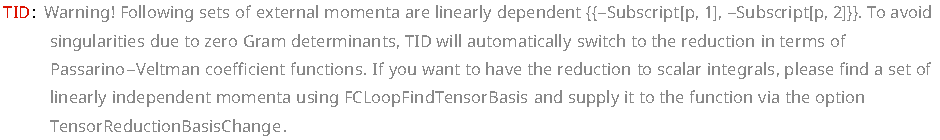
\includegraphics[width=0.6\linewidth]{img/1d92pz2yqj2pc.pdf}
\end{figure}
\FloatBarrier

\begin{dmath*}\breakingcomma
-i \pi ^2 \left(p_1{}^{\mu }+p_2{}^{\mu }\right) \;\text{C}_1\left(0,M^2,M^2,0,0,m^2\right)
\end{dmath*}

A vanishing Gram determinant signals that the external momenta are
linearly dependent on each other. This redundancy can be resolved by
switching to a different basis. To that aim we need to run
\texttt{FCLoopFindTensorBasis} to analyze the set of external momenta
causing troubles

\begin{Shaded}
\begin{Highlighting}[]
\NormalTok{FCLoopFindTensorBasis}\OperatorTok{[\{}\SpecialCharTok{{-}}\FunctionTok{Subscript}\OperatorTok{[}\FunctionTok{p}\OperatorTok{,} \DecValTok{1}\OperatorTok{],} \SpecialCharTok{{-}}\FunctionTok{Subscript}\OperatorTok{[}\FunctionTok{p}\OperatorTok{,} \DecValTok{2}\OperatorTok{]\},} \OperatorTok{\{\},} \FunctionTok{n}\OperatorTok{]}
\end{Highlighting}
\end{Shaded}

\begin{dmath*}\breakingcomma
\left(
\begin{array}{c}
 -p_1 \\
 -p_2 \\
 -p_2\to -p_1 \;\text{FCGV}(\text{Prefactor})(1) \\
\end{array}
\right)
\end{dmath*}

We see that \(p_1\) and \(p_2\) are proportional to each other, so that
only one of these vectors is linearly independent. This also means that
the scalar products involving loop momentum \(p_1 \cdot k\) and
\(p_2 \cdot k\) are identical. Supplying this information to
\texttt{TID} we can now achieve the desired reduction to scalars.

\begin{Shaded}
\begin{Highlighting}[]
\NormalTok{TID}\OperatorTok{[}\NormalTok{FAD}\OperatorTok{[\{}\FunctionTok{k}\OperatorTok{,} \FunctionTok{m}\OperatorTok{\},} \FunctionTok{k} \SpecialCharTok{{-}} \FunctionTok{Subscript}\OperatorTok{[}\FunctionTok{p}\OperatorTok{,} \DecValTok{1}\OperatorTok{],} \FunctionTok{k} \SpecialCharTok{{-}} \FunctionTok{Subscript}\OperatorTok{[}\FunctionTok{p}\OperatorTok{,} \DecValTok{2}\OperatorTok{]]}\NormalTok{ FVD}\OperatorTok{[}\FunctionTok{k}\OperatorTok{,} \SpecialCharTok{\textbackslash{}}\OperatorTok{[}\NormalTok{Mu}\OperatorTok{]],} \FunctionTok{k}\OperatorTok{,} 
\NormalTok{  TensorReductionBasisChange }\OtherTok{{-}\textgreater{}} \OperatorTok{\{\{}\SpecialCharTok{{-}}\FunctionTok{Subscript}\OperatorTok{[}\FunctionTok{p}\OperatorTok{,} \DecValTok{1}\OperatorTok{],} \SpecialCharTok{{-}}\FunctionTok{Subscript}\OperatorTok{[}\FunctionTok{p}\OperatorTok{,} \DecValTok{2}\OperatorTok{]\}} \OtherTok{{-}\textgreater{}} \OperatorTok{\{}\SpecialCharTok{{-}}\FunctionTok{Subscript}\OperatorTok{[}\FunctionTok{p}\OperatorTok{,} \DecValTok{1}\OperatorTok{]\}\},} 
\NormalTok{  FinalSubstitutions }\OtherTok{{-}\textgreater{}} \OperatorTok{\{}\NormalTok{SPD}\OperatorTok{[}\FunctionTok{k}\OperatorTok{,} \FunctionTok{Subscript}\OperatorTok{[}\FunctionTok{p}\OperatorTok{,} \DecValTok{2}\OperatorTok{]]} \OtherTok{{-}\textgreater{}}\NormalTok{ SPD}\OperatorTok{[}\FunctionTok{k}\OperatorTok{,} \FunctionTok{Subscript}\OperatorTok{[}\FunctionTok{p}\OperatorTok{,} \DecValTok{1}\OperatorTok{]]\}]}
\end{Highlighting}
\end{Shaded}

\begin{dmath*}\breakingcomma
\frac{\left((m-M) (m+M)+2 M^2\right) p_1{}^{\mu }}{2 M^2 \left(k^2\right)^2.\left((k+p_1){}^2-m^2\right)}-\frac{p_1{}^{\mu }}{2 M^2 k^2.\left((k+p_1){}^2-m^2\right)}
\end{dmath*}

Notice that the result contains a propagator squared. This can be
reduced further using IBPs (e.g.~by employing FIRE or KIRA via the
FeynHelpers interface).

For cases involving light-like external momenta we often need to
introduce an auxiliary vector, since the available vector are not
sufficient to form a basis

\begin{Shaded}
\begin{Highlighting}[]
\NormalTok{FCClearScalarProducts}\OperatorTok{[]}\NormalTok{; }
 
\NormalTok{SPD}\OperatorTok{[}\FunctionTok{p}\OperatorTok{]} \ExtensionTok{=} \DecValTok{0}\NormalTok{; }
 
\NormalTok{TID}\OperatorTok{[}\NormalTok{FAD}\OperatorTok{[\{}\FunctionTok{k}\OperatorTok{,} \FunctionTok{m}\OperatorTok{\},} \FunctionTok{k} \SpecialCharTok{{-}} \FunctionTok{p}\OperatorTok{]}\NormalTok{ FVD}\OperatorTok{[}\FunctionTok{k}\OperatorTok{,} \SpecialCharTok{\textbackslash{}}\OperatorTok{[}\NormalTok{Mu}\OperatorTok{]],} \FunctionTok{k}\OperatorTok{]}
\end{Highlighting}
\end{Shaded}

\FloatBarrier
\begin{figure}[!ht]
\centering
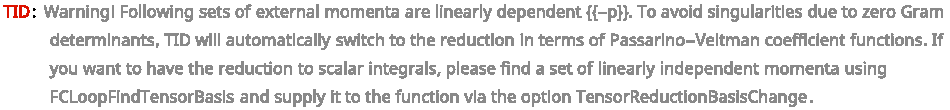
\includegraphics[width=0.6\linewidth]{img/0kz04gd9tjslc.pdf}
\end{figure}
\FloatBarrier

\begin{dmath*}\breakingcomma
\frac{p^{\mu }}{k^2.\left((k-p)^2-m^2\right)}+i \pi ^2 p^{\mu } \;\text{B}_1\left(0,0,m^2\right)
\end{dmath*}

Running \texttt{FCLoopFindTensorBasis} we get a suggestion to introduce
an auxiliary vector \(n\) to the basis. The scalar products of this
vector with other external momenta must be nonvanishing, but we are free
to make the vector itself light-like (for simplicity)

\begin{Shaded}
\begin{Highlighting}[]
\NormalTok{FCLoopFindTensorBasis}\OperatorTok{[\{}\SpecialCharTok{{-}}\FunctionTok{p}\OperatorTok{\},} \OperatorTok{\{\},} \FunctionTok{n}\OperatorTok{]}
\end{Highlighting}
\end{Shaded}

\begin{dmath*}\breakingcomma
\{\{-p,n\},\{\},\{\}\}
\end{dmath*}

\begin{Shaded}
\begin{Highlighting}[]
\NormalTok{SPD}\OperatorTok{[}\FunctionTok{n}\OperatorTok{]} \ExtensionTok{=} \DecValTok{0}\NormalTok{; }
 
\NormalTok{TID}\OperatorTok{[}\NormalTok{FAD}\OperatorTok{[\{}\FunctionTok{k}\OperatorTok{,} \FunctionTok{m}\OperatorTok{\},} \FunctionTok{k} \SpecialCharTok{{-}} \FunctionTok{p}\OperatorTok{]}\NormalTok{ FVD}\OperatorTok{[}\FunctionTok{k}\OperatorTok{,} \SpecialCharTok{\textbackslash{}}\OperatorTok{[}\NormalTok{Mu}\OperatorTok{]],} \FunctionTok{k}\OperatorTok{,}\NormalTok{ TensorReductionBasisChange }\OtherTok{{-}\textgreater{}} \OperatorTok{\{\{}\SpecialCharTok{{-}}\FunctionTok{p}\OperatorTok{\}} \OtherTok{{-}\textgreater{}} \OperatorTok{\{}\SpecialCharTok{{-}}\FunctionTok{p}\OperatorTok{,} \FunctionTok{n}\OperatorTok{\}\},}\NormalTok{ AuxiliaryMomenta }\OtherTok{{-}\textgreater{}} \OperatorTok{\{}\FunctionTok{n}\OperatorTok{\}]}
\end{Highlighting}
\end{Shaded}

\begin{dmath*}\breakingcomma
\frac{-2 p^{\mu } (k\cdot n)+m^2 n^{\mu }+2 p^{\mu } (n\cdot p)}{2 (n\cdot p) k^2.\left((k-p)^2-m^2\right)}-\frac{n^{\mu }}{2 (n\cdot p) \left(k^2-m^2\right)}
\end{dmath*}

Unfortunately, in this case \texttt{TID} alone cannot eliminate the
scalar products of \(n\) with the loop momentum in the numerator. For
that we need to use IBPs. Still, it manages to reduce the tensor
integral to scalars, even though at this stage not all of them can be
mapped to scalar PaVe functions.

The dependence on the auxiliary vector \(n\) must cancel in the final
result for this integral, as the auxiliary vector is unphysical and the
original integral does not depend on it. To arrive at these
cancellations for more complicated tensor integral it might be necessary
to exploit the relations between the physical vectors as given by
\texttt{FCLoopFindTensorBasis} and contract those with \(n\).

In FeynCalc, Passarino-Veltman coefficient functions are defined in the
same way as in LoopTools. If one wants to use a different definition, it
is useful to activate the option GenPaVe

\begin{Shaded}
\begin{Highlighting}[]
\NormalTok{FCClearScalarProducts}\OperatorTok{[]}\NormalTok{; }
 
\NormalTok{SPD}\OperatorTok{[}\FunctionTok{Subscript}\OperatorTok{[}\FunctionTok{p}\OperatorTok{,} \DecValTok{1}\OperatorTok{],} \FunctionTok{Subscript}\OperatorTok{[}\FunctionTok{p}\OperatorTok{,} \DecValTok{1}\OperatorTok{]]} \ExtensionTok{=} \DecValTok{0}\NormalTok{; }
 
\NormalTok{SPD}\OperatorTok{[}\FunctionTok{Subscript}\OperatorTok{[}\FunctionTok{p}\OperatorTok{,} \DecValTok{2}\OperatorTok{],} \FunctionTok{Subscript}\OperatorTok{[}\FunctionTok{p}\OperatorTok{,} \DecValTok{2}\OperatorTok{]]} \ExtensionTok{=} \DecValTok{0}\NormalTok{; }
 
\NormalTok{SPD}\OperatorTok{[}\FunctionTok{Subscript}\OperatorTok{[}\FunctionTok{p}\OperatorTok{,} \DecValTok{1}\OperatorTok{],} \FunctionTok{Subscript}\OperatorTok{[}\FunctionTok{p}\OperatorTok{,} \DecValTok{2}\OperatorTok{]]} \ExtensionTok{=} \DecValTok{0}\NormalTok{; }
 
\NormalTok{TID}\OperatorTok{[}\NormalTok{FAD}\OperatorTok{[\{}\FunctionTok{k}\OperatorTok{,} \FunctionTok{m}\OperatorTok{\},} \FunctionTok{k} \SpecialCharTok{{-}} \FunctionTok{Subscript}\OperatorTok{[}\FunctionTok{p}\OperatorTok{,} \DecValTok{1}\OperatorTok{],} \FunctionTok{k} \SpecialCharTok{{-}} \FunctionTok{Subscript}\OperatorTok{[}\FunctionTok{p}\OperatorTok{,} \DecValTok{2}\OperatorTok{]]}\NormalTok{ FVD}\OperatorTok{[}\FunctionTok{k}\OperatorTok{,} \SpecialCharTok{\textbackslash{}}\OperatorTok{[}\NormalTok{Mu}\OperatorTok{]]} \SpecialCharTok{//}\NormalTok{ FCI}\OperatorTok{,} \FunctionTok{k}\OperatorTok{,}\NormalTok{ GenPaVe }\OtherTok{{-}\textgreater{}} \ConstantTok{True}\OperatorTok{]} 
 
\NormalTok{FCClearScalarProducts}\OperatorTok{[]}\NormalTok{;}
\end{Highlighting}
\end{Shaded}

\FloatBarrier
\begin{figure}[!ht]
\centering
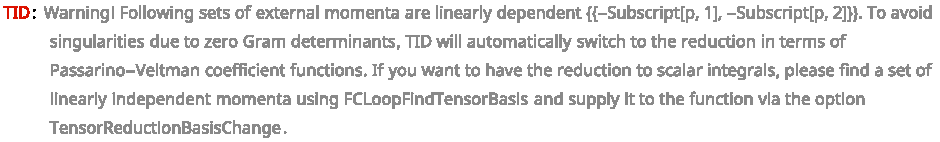
\includegraphics[width=0.6\linewidth]{img/1mx6pq1c6qsv5.pdf}
\end{figure}
\FloatBarrier

\begin{dmath*}\breakingcomma
-i \pi ^2 p_1{}^{\mu } \;\text{GenPaVe}\left(\{1\},\left(
\begin{array}{cc}
 0 & m \\
 p_1 & 0 \\
 p_2 & 0 \\
\end{array}
\right)\right)-i \pi ^2 p_2{}^{\mu } \;\text{GenPaVe}\left(\{2\},\left(
\begin{array}{cc}
 0 & m \\
 p_1 & 0 \\
 p_2 & 0 \\
\end{array}
\right)\right)
\end{dmath*}

To simplify manifestly IR-finite 1-loop results written in terms of
Passarino-Veltman functions, we may employ the option
\texttt{PaVeLimitTo4} (must be used together with \texttt{ToPaVe}). The
result is valid up to 0th order in \texttt{Epsilon}, i.e.~sufficient for
1-loop calculations.

\begin{Shaded}
\begin{Highlighting}[]
\NormalTok{FCClearScalarProducts}\OperatorTok{[]}\NormalTok{; }
 
\NormalTok{int }\ExtensionTok{=}\NormalTok{ (}\FunctionTok{D} \SpecialCharTok{{-}} \DecValTok{1}\NormalTok{) (}\FunctionTok{D} \SpecialCharTok{{-}} \DecValTok{2}\NormalTok{)}\SpecialCharTok{/}\NormalTok{(}\FunctionTok{D} \SpecialCharTok{{-}} \DecValTok{3}\NormalTok{) FVD}\OperatorTok{[}\FunctionTok{p}\OperatorTok{,}\NormalTok{ mu}\OperatorTok{]}\NormalTok{ FVD}\OperatorTok{[}\FunctionTok{p}\OperatorTok{,}\NormalTok{ nu}\OperatorTok{]}\NormalTok{ FAD}\OperatorTok{[}\FunctionTok{p}\OperatorTok{,} \FunctionTok{p} \SpecialCharTok{{-}} \FunctionTok{q}\OperatorTok{]}
\end{Highlighting}
\end{Shaded}

\begin{dmath*}\breakingcomma
\frac{(D-2) (D-1) p^{\text{mu}} p^{\text{nu}}}{(D-3) p^2.(p-q)^2}
\end{dmath*}

\begin{Shaded}
\begin{Highlighting}[]
\NormalTok{TID}\OperatorTok{[}\NormalTok{int}\OperatorTok{,} \FunctionTok{p}\OperatorTok{,}\NormalTok{ ToPaVe }\OtherTok{{-}\textgreater{}} \ConstantTok{True}\OperatorTok{]}
\end{Highlighting}
\end{Shaded}

\begin{dmath*}\breakingcomma
\frac{i \pi ^2 (2-D) \;\text{B}_0\left(q^2,0,0\right) \left(D q^{\text{mu}} q^{\text{nu}}-q^2 g^{\text{mu}\;\text{nu}}\right)}{4 (3-D)}
\end{dmath*}

\begin{Shaded}
\begin{Highlighting}[]
\NormalTok{TID}\OperatorTok{[}\NormalTok{int}\OperatorTok{,} \FunctionTok{p}\OperatorTok{,}\NormalTok{ ToPaVe }\OtherTok{{-}\textgreater{}} \ConstantTok{True}\OperatorTok{,}\NormalTok{ PaVeLimitTo4 }\OtherTok{{-}\textgreater{}} \ConstantTok{True}\OperatorTok{]}
\end{Highlighting}
\end{Shaded}

\begin{dmath*}\breakingcomma
\frac{1}{2} i \pi ^2 \;\text{B}_0\left(\overline{q}^2,0,0\right) \left(4 \overline{q}^{\text{mu}} \overline{q}^{\text{nu}}-\overline{q}^2 \bar{g}^{\text{mu}\;\text{nu}}\right)+\frac{1}{2} i \pi ^2 \left(2 \overline{q}^{\text{mu}} \overline{q}^{\text{nu}}-\overline{q}^2 \bar{g}^{\text{mu}\;\text{nu}}\right)
\end{dmath*}

Sometimes one would like to have external momenta multiplied by symbolic
parameters in the propagators. In this case one should first declare the
corresponding variables to be of \texttt{FCVariable} type

\begin{Shaded}
\begin{Highlighting}[]
\NormalTok{DataType}\OperatorTok{[}\FunctionTok{a}\OperatorTok{,}\NormalTok{ FCVariable}\OperatorTok{]} \ExtensionTok{=} \ConstantTok{True}\NormalTok{;}
\NormalTok{DataType}\OperatorTok{[}\FunctionTok{b}\OperatorTok{,}\NormalTok{ FCVariable}\OperatorTok{]} \ExtensionTok{=} \ConstantTok{True}\NormalTok{;}
\end{Highlighting}
\end{Shaded}

\begin{Shaded}
\begin{Highlighting}[]
\NormalTok{ExpandScalarProduct}\OperatorTok{[}\NormalTok{SP}\OperatorTok{[}\FunctionTok{P}\OperatorTok{,} \FunctionTok{Q}\OperatorTok{]} \OtherTok{/.} \FunctionTok{P} \OtherTok{{-}\textgreater{}} \FunctionTok{a}\NormalTok{ P1 }\SpecialCharTok{+} \FunctionTok{b}\NormalTok{ P2}\OperatorTok{]} 
 
\FunctionTok{StandardForm}\OperatorTok{[}\SpecialCharTok{\%}\OperatorTok{]}

\NormalTok{\textasciigrave{}\textasciigrave{}\textasciigrave{}mathematica}

\NormalTok{$$a }\SpecialCharTok{\textbackslash{}}\FunctionTok{left}\NormalTok{(}\SpecialCharTok{\textbackslash{}}\NormalTok{overline}\OperatorTok{\{}\SpecialCharTok{\textbackslash{}}\FunctionTok{text}\OperatorTok{\{}\NormalTok{P1}\OperatorTok{\}\}}\SpecialCharTok{\textbackslash{}}\NormalTok{cdot }\SpecialCharTok{\textbackslash{}}\NormalTok{overline}\OperatorTok{\{}\FunctionTok{Q}\OperatorTok{\}}\SpecialCharTok{\textbackslash{}}\FunctionTok{right}\NormalTok{)}\SpecialCharTok{+}\FunctionTok{b} \SpecialCharTok{\textbackslash{}}\FunctionTok{left}\NormalTok{(}\SpecialCharTok{\textbackslash{}}\NormalTok{overline}\OperatorTok{\{}\SpecialCharTok{\textbackslash{}}\FunctionTok{text}\OperatorTok{\{}\NormalTok{P2}\OperatorTok{\}\}}\SpecialCharTok{\textbackslash{}}\NormalTok{cdot }\SpecialCharTok{\textbackslash{}}\NormalTok{overline}\OperatorTok{\{}\FunctionTok{Q}\OperatorTok{\}}\SpecialCharTok{\textbackslash{}}\FunctionTok{right}\NormalTok{)$$}

\NormalTok{\textasciigrave{}\textasciigrave{}\textasciigrave{}mathematica}
\CommentTok{(*a Pair[Momentum[P1], Momentum[Q]] + b Pair[Momentum[P2], Momentum[Q]]*)}
\end{Highlighting}
\end{Shaded}

\end{document}
